\subsection{Приклади дослідження на стійкість диф. рівнянь, що описують поведінку екологічних процесів.}

\subsubsection{Модель одновимірної популяції.}

Однією з важливих проблем екології є динаміка чисельності популяції. Нехай маємо популяцію, що складається з особин одного виду, знайдемо закон зміни її чисельності.\\

Припустимо, що: існують лише процеси розмноження та смерті, швидкості яких пропорційні кількості особин в даний момент часу; не враховується внутрішньовидова боротьба; розглядаємо лише одну популяцію (відсутність хижаки). \\

$x(t) - $ кількість особин в момент $t$.\\
$R - $ швидкість розмноження. \\
$\gamma - $ коефіцієнт розмноження. \\
$ R = \gamma x $\\
$ S - $ швидкість природньої загибелі.\\
$\sigma - $ коефіцієнт смертності (природньої).\\
$S = - rx$\\
Тоді: $ \frac{dx}{dt} = \gamma x - \sigma x = (\gamma - \sigma)x $.\\
Позначення: $ \gamma - \sigma = a$. Тоді \fbox{$    \frac{dx}{dt} = ax $} - закон Мальтуса.
\begin{center} 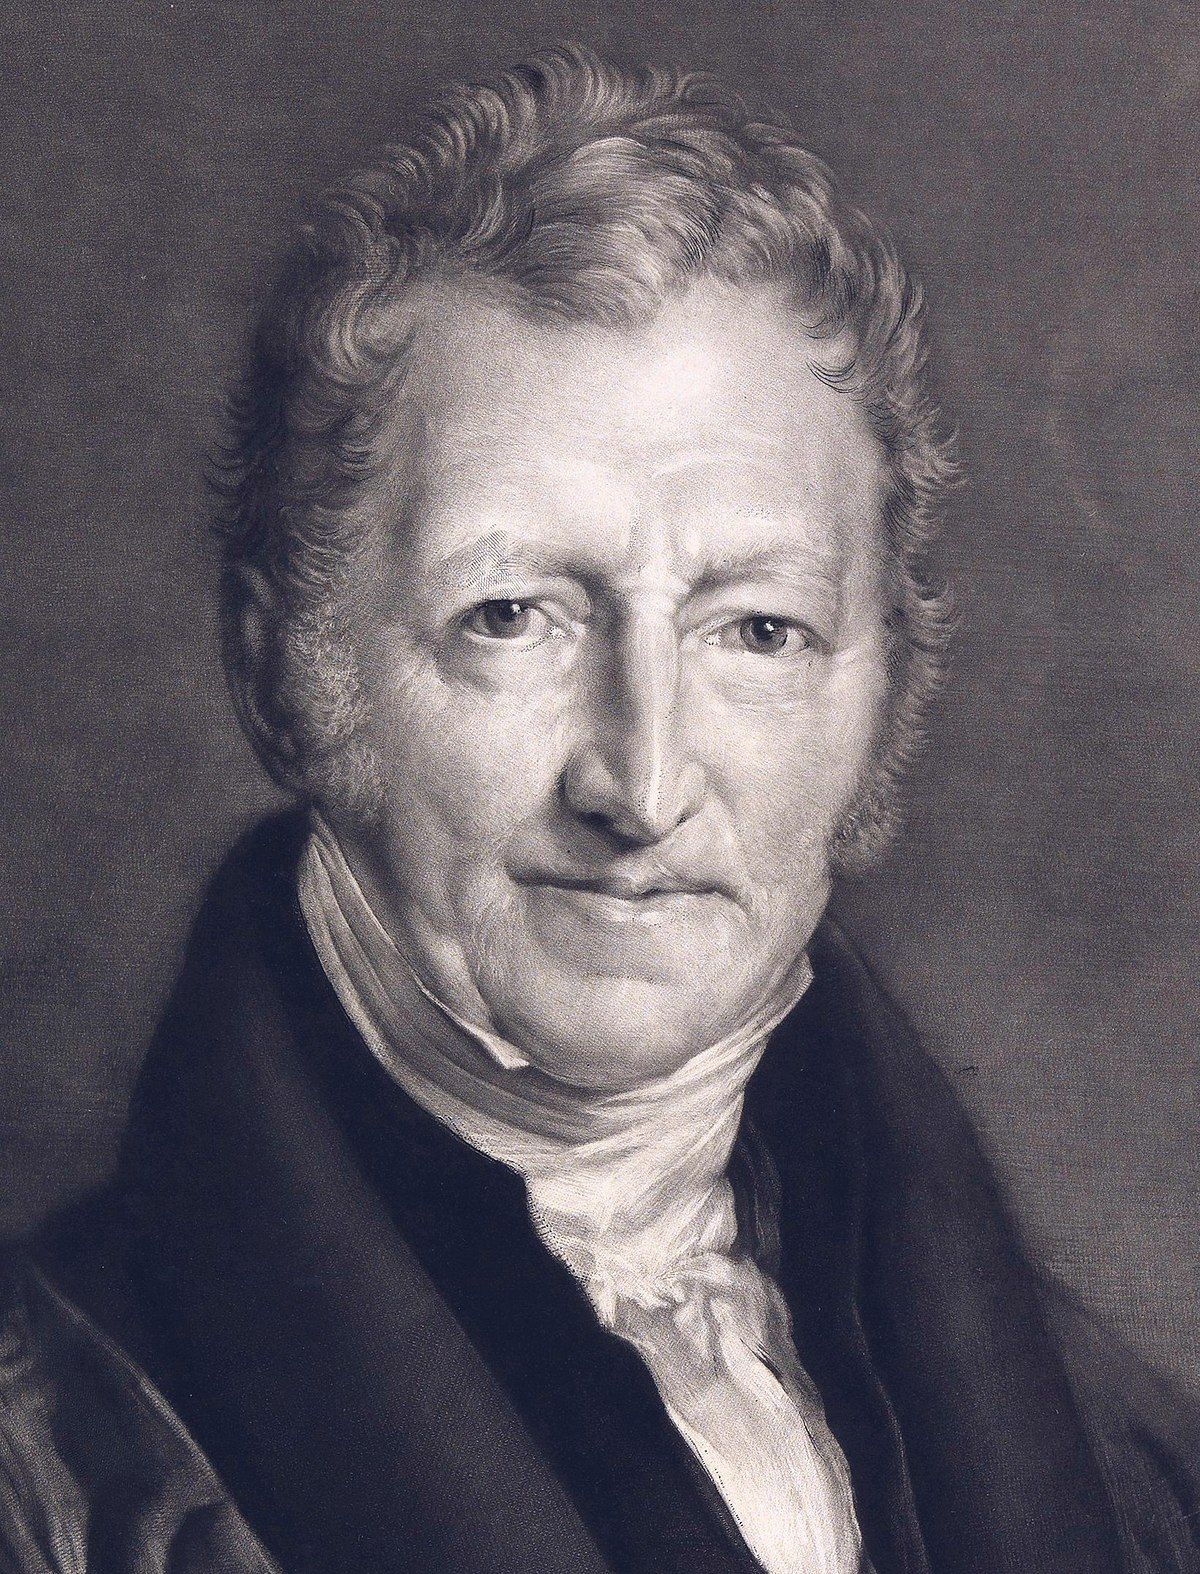
\includegraphics[scale=0.1]{assets/lectures_recent-44a47cac.png} \end{center}

Томас Мальтус (1766-1834), - англ. вчений, демограф, економіст, священик;\\
1798 р.:''Все про принципи народонаселення.''
$$
\frac{dx}{dt} = ax \Longrightarrow x(t) = C \cdot e^{at} - \text{загальний розв'язок.}
$$
Нехай в початковий момент часу $t_0 = 0$ кількість особин складає $x_0$ особин:
$$
x(0) = x_0
$$
Тоді: $x(t) = x_0 \cdot e^{at} $ - розв'язок даної задачі Коші. Розглянемо випадки:

а) $a < 0$ (помирають більше, ніж народжується). Оскільки дане рівняння - лінійне, то всі розв'язки водночас стійкі (нест., ас. ст.). Тому дослідимо на стійкість розв'язок $ \varphi(t) = 0$ (умова 1 стійкості виконується); розв'язок довільної задачі К.:
$$
x(t_0) = x_0 : x(t) = x_0 e^{a (t-t_0)}
$$
Нехай $ \left| x_0 \right| < \delta.$ Розглянемо:
$$
\forall t \geq t_0 \quad \left| x (t) \right| = \underbrace{e^{a(t-t_0)}}_{<1, \text{ при } t\geq t_0} \left| x_0 \right| \xrightarrow[t\to + \infty]{} 0 < \varepsilon \text{ при } \varepsilon = \delta
$$
$\Rightarrow $ всі розв'язки рівняння асимптотично стійкі та прямують до нуля.\\
\begin{center} 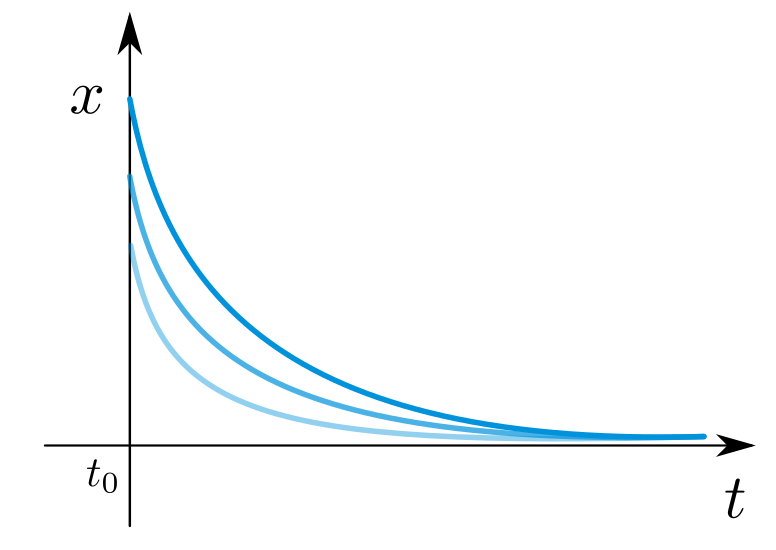
\includegraphics[scale=0.2]{assets/lectures_recent-562c17da.png} \end{center}
Це означає, що якою б великою не була кількість особин в початковий момент часу, якщо смертність перевищує народжуваність, кількість особин з часом прямує до 0 ($t \to + \infty$).
